
\documentclass[tikz,border=2pt]{standalone}
\usepackage{tikz}
\usepackage{lmodern}
\usetikzlibrary{calc,decorations.pathreplacing}

% Visual conventions follow the existing MRNC TikZ pictures: ordinary
% components use TikZ's normal 0.4pt stroke, with compact TeX labels.
\tikzset{
  nu fibre/.style={
    x=0.78cm,
    y=0.78cm,
    line width=0.4pt,
    line cap=round,
    line join=round
  },
  nu label/.style={
    font=\scriptsize,
    inner sep=1pt
  },
  nu annotation/.style={
    font=\scriptsize,
    inner sep=1pt
  },
  nu dots/.style={
    font=\small,
    inner sep=0pt
  }
}

\begin{document}

% III-II_{l+1}^*


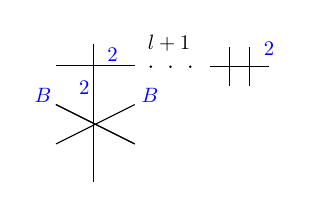
\begin{tikzpicture}[scale=0.5]
  % Coordinates
  \coordinate (A) at (-2.95, 3.57);
  \coordinate (B) at (-2.95, 0.07);
  \coordinate (E) at (-3.91, 1.04);
  \coordinate (F) at (-1.91, 2.04);
  \coordinate (G) at (-3.91, 2.04);
  \coordinate (H) at (-1.91, 1.04);
  \coordinate (C) at (-3.91, 3.04);
  \coordinate (D) at (-1.91, 3.04);
  \coordinate (I) at (-1.50, 3.00);
  \coordinate (J) at (-1.00, 3.00);
  \coordinate (K) at (-0.50, 3.00);
  \coordinate (N) at (0.50, 3.50);
  \coordinate (O) at (0.50, 2.50);
  \coordinate (P) at (1.00, 3.50);
  \coordinate (Q) at (1.00, 2.50);
  \coordinate (L) at (0.00, 3.00);
  \coordinate (M) at (1.50, 3.00);
  \coordinate (R) at (-1.04, 3.22);
  \coordinate (S) at (-4.24, 1.90);
  \coordinate (T) at (-1.52, 1.90);
  \coordinate (U) at (1.5, 3.10);
  \coordinate (V) at (-3.19, 2.10);
  \coordinate (W) at (-2.47, 2.95);

  % Drawing
  \draw (A) -- (B);
  \draw (C) -- (D);
  \draw (G) -- (H);
  \draw (E) -- (F);
  \draw (G) -- (H);
  \draw (C) -- (D);
  \draw (N) -- (O);
  \draw (P) -- (Q);
  \draw (L) -- (M);
  \node[scale=0.75][above] at (R) {$l+1
$};
  \node[scale=0.75][above, text=blue] at (S) {$B$};
  \node[scale=0.75][above, text=blue] at (T) {$B$};
  \node[scale=0.75][above, text=blue] at (U) {$2
$};
  \node[scale=0.75][above, text=blue] at (V) {$2$};
  \node[scale=0.75][above, text=blue] at (W) {$2$};
  \fill[black] (I) circle (1pt);
  \fill[black] (J) circle (1pt);
  \fill[black] (K) circle (1pt);
\end{tikzpicture}

\end{document}
